\chapter{Štandardy BSI: IT-Grundshutz}
\label{chap:it-grundschutz}
\emph{Bundesamt für Sicherheit in der Informationstechnik} (BSI), je nemecká federálna agentúra,
ktorá zodpovedá za kybernetickú bezpečnosť a bezpečnú digitalizáciu Nemeckej spolkovej republiky\cite{bsibundde}.
BSI vypracoval a od roku 1990 rozvíja systematické riešenie (ISMS) pre informačnú bezpečnosť rôznych organizácií,
ktorý nazval IT-Grundschutz (z nem. jazyka, v preklade základná ochrana IT). Metodika zavádzania systému informačnej
bezpečnosti (ISMS, viac v kapitole \nameref{chap:isms}) a kontinuálneho manažmentu informačnej bezpečnosti je rozpracovaná
v nasledovných publikáciach BSI:

\begin{itemize}[nosep]
    \item BSI Standard 200-1 \cite{BSI1}, základné požiadavky ISMS
    \item BSI Standard 200-2 \cite{BSI2}, postup zavedenia ISMS
    \item BSI Standard 200-3 \cite{BSI3}, analýzu rizík
    \item BSI Standard 100-4 \cite{BSI4}, manažment kontinuity
    \item IT-Grundshutz Kompendium \cite{GSK}, katalóg modulov pre rozličné oblasti
\end{itemize}

IT-Grundschutz je kompatibilný s medzinárodným štandardom ISO/IEC 27000 a organizácie môžu svoj systém manažmentu
informačnej bezpečnosti certifikovať podľa ISO 27001. V prípade organizácie pôsobiacu na Slovensku alebo štátnu
inštitúciu môže byť vhodné nasledovať IT-Grundschutz, keďže certifikovať sa podľa ISO 27001 prakticky znamená splniť
požiadavky vyplývajúce z \cite{ZoKB} alebo \cite{ZoITVS}\footnote{Skutočnosti, že oba zákony sú postavené na štandardoch
ISO/IEC 27000, sme sa venovali v bakalárskej práci.}.


\section{Filozofia štandardov BSI}
\label{sec:bsiphilosophy}

Štandardy BSI presadzujú tzv. holistický koncept informačnej bezpečnosti\footnote{Prívlastok holistický, resp.
holizmus ako filozofický smer vychádza z presvedčenia, že skutočnosť môžme pochopiť iba ako väčší celok --- celok
je viac, ako súčet jeho častí. Ide o opak redukcionizmu, ktorý vysvetľuje zložité skutočnosti jej rozkladom na 
jednoduchšie ľahko pochopiteľné časti \cite{WikiHolism}.}. Aby sme zaistili efektívnu informačnú bezpečnosť, musíme ju
presadzovať na každej úrovni organizácie (počnúc vedením, cez procesy, zamestnancov až po samotné IT systémy a zariadenia).
Spolkový úrad BSI analyzovala typické organizácie a identifikoval spoločné úlohy, procesy, problémy a ďalšie
spoločné prvky, súvisiace s riešením informačnej bezpečnosti a došiel k záveru, že malé a stredne veľké organizácie
nemajú potrebné \enquote{know-how}, ľudské ani finančne zdroje na zaistenie potrebnej úrovne informačnej bezpečnosti v
jednom kroku\cite{BSI1}. Organizáciám, ktoré sú v tejto nepriaznivej situácii, sa úrad BSI snaží pomôcť. 

Vo vyššie uvedených publikáciach predkladá čitateľovi\footnote{Zamestnancovi poverenému informačnou bezpečnosťou.} 
podrobný návod na implementáciu systému základných (nevyhnutných) bezpečnostných opatrení. Štandardy rozoberajú rôzne
príklady, kladú otázky a ponúkajú potenciálne odpovede, aby vhodne usmernili/pomohli procesu zavádzania/správy
informačnej bezpečnosti. Vďaka takémuto prístupu môže aj zamestnanec so základnou znalosťou informatiky pozdvihnúť
úroveň informačnej bezpečnosti v organizácii na požadovanú\footnote{Požadovanú v zmysle relevantného zákona alebo
štandardu pre účely certifikácie.} úroveň. 

Keďže slovenské organizácie narážajú (v informačnej bezpečnosti) na podobné problémy, ako nemecké a mnohé z nich sú zo
zákona (ZoITVS) povinné zaviesť systém manažmentu informačnej bezpečnosti, ISMS, môžu využívať riešenia, ktoré ponúka
nemecký IT-Grundschutz. V nasledujúcej časti zjednodušene popíšeme proces, ktorým môžeme zaviesť ISMS a systematicky 
riešiť informačnú bezpečnosť v organizácií. Naším cieľom je vysvetliť čitateľovi (v prvom rade manažérovi kybernetickej
a informačnej bezpečnosti) podstatu, význam a spôsoby realizácie analýzy rizík do takej miery, aby bol schopný analyzovať,
vyhodnotiť a ošetriť bezpečnostné riziká svojej organizácie.

V nasledujúcej časti zjednodušene popíšeme proces, ktorým môžeme systematicky zaviesť informačnú bezpečnosť v organizácií.
Naším konečným cieľom je ukotviť analýzu rizík v kontexte tohto procesu.

\section{System riadenia informačnej bezpečnosti --- ISMS}
\label{sec:isms}

Informačne systémy sa nachádzajú v neustále meniacom sa kybernetickom priestore. Z tejto inherentnej vlastnosti vyplýva, že proces
KIB musíme kontinuálne prispôsobovať zmenám, aby zostal aktuálny, efektívny a účinný. Manažérsky proces, ktorý formalizuje
a zastrešuje celý proces riadenia informačnej bezpečnosti v organizácii nazývame ISMS (z angl. \emph{information securuity
management system}). Keďže ide o kľúčový pojem, ktorý však (v ISO normách ani v slovenskej legislatíve) nie je zrozumiteľne
vysvetlený (a pritom organizácia by ISMS mala zaviesť), uvedieme popis ISMS tak, ako ho uvádzajú štandardy BSI.

Základné požiadavky na ISMS, definované ISO normou ISO/IEC 27001, vysvetľuje  Štandard \cite{BSI1}. ISMS pozostáva zo štyroch
komponentov zobrazených na obrázku \ref{fig:isms-bsi1}, pri každom z komponentov sú v bodoch zhrnuté jeho kľúčové aspekty. 
V krátkosti priblížime význam jednotlivých komponentov. 

\input tikz/isms-bsi1.tex

\textbf{Manažerské princípy} sa týkajú najmä vedenia organizácie, ktorého úlohou je explicitne ustanoviť proces KIB, ako vedomú
a cielenú činnosť naprieč celou organizáciou. Vedenie musí vytvoriť stratégiu KIB, v ktorej jasne určí svoje
ciele\footnote{Tieto ciele možu vyplývať z poslania a procesov organizácie, ale aj zo zákonných povinností.} KIB, a ako ich
plánuje naplniť. Vedenie musí vytvoriť rolu manažéra KIB, ktorého úlohou je riadiť ISMS a komunikovať dôležité
informácie/rozhodnutia/problémy s vedením organizácie.

\textbf{Finančné/personálne/časové zdroje} sú potrebné na efektívne splnenie cieľov KIB. Vedenie potrebuje
nastaviť realistické ciele a na ich splnenie vymedziť potrebné zdroje. Vedenie tiež musí byť schopné robiť informované rozhodnutia,
aby zbytočne neplytvalo týmito zdrojmi (ako sú drahé technické riešenie, prehnané administratívne zaťaženie
alebo časovo-zdĺhavá implementácia opatrenia).

\textbf{Zamesntanci} sú neoddeliteľnou súčasťou organizácie, a preto sa musia aktívne zapájať do KIB. Každý zamestnanec je
zaradený do roly KIB a musí vedieť, aké má povinnosti, ktoré zručnosti potrebuje mať a aké negatívne dôsledky môže mať
jeho správanie.

\textbf{Bezpečnostný proces} slúži na udržiavanie primeranej úrovne KIB v organizácií. Riadi sa tzv.
PDCA(\emph{angl. “Plan”, “Do”, “Check”, “Act”}) cyklom. Organizácia urči svoj stav a podmienky,
v ktorých sa nachádza (napr. poslanie a štruktúra organizácie, strategický kontext alebo zainteresované
tretie strany). Na základe týchto vstupov organizácia pomenuje bezpečnostné ciele a vypracuje politiku KIB, ktorá popisuje
význam KIB a určuje povinnosti v KIB. Ciele a politika KIB sú ďalej rozvinuté a implementované pomocou koncepcie KIB.
Nakoniec organizácia posudzuje výkonnosť a efektívnosť bezpečnostného procesu (metriky, audit) a pravidelne zdokonaľuje určené
ciele, politiku a koncepciu KIB.

IT-Grundschutz poskytuje tri úrovne prístupu k ochrane aktív: základný (\emph{basic}), jadrový (\emph{core}) a štandardný
(\emph{standard}). Voľba prístupu závisí od identifikovaných bezpečnostných požiadaviek.

\textbf{Základná ochrana} formuje základy informačnej bezpečnosti, jej hlavným účelom je zaviesť základné bezpečnostné opatrenia,
ktoré majú široký dosah na aktíva organizácie. Ich zavedenie si vyžaduje pomerne malé úsilie, a preto základnú ochranu vieme
pomerne rýchlo implementovať. 

\textbf{Jadrová ochrana} sústreďuje pozornosť na tzv. klenoty organizácie, ktorých narušenie môže ohrozovať existenciu organizácie. 

\textbf{Štandardná ochrana} slúži na komplexnú ochranu všetkých častí organizácie, vyžaduje si ale väčšiu dávku úsilia a
väčšie množstvo zdrojov. Na obrázku \ref{fig:securuity-concept-bsi2} môžeme vidieť náčrt bezpečnostného konceptu pre
{\color{NavyBlue}základnú (modrá)}, {\color{Orange}jadrovú (oranžová)} a {\color{Green}štandardnú (zelená)} ochranu,
pre ľahšie porovnanie vzájomných rozdielov sme ich uložili vedľa seba.

\newcommand{\fourarrows}[2]{%
    \draw[arr] ([xshift=-2.25cm]#1) -- ([xshift=-2.25cm]#2);
    \draw[arr] ([xshift=-0.75cm]#1) -- ([xshift=-0.75cm]#2);
    \draw[arr] ([xshift=0.75cm]#1) -- ([xshift=0.75cm]#2);
    \draw[arr] ([xshift=2.25cm]#1) -- ([xshift=2.25cm]#2);
};
 
\begin{figure}[ht]
    \centering
    \begin{tikzpicture}[
        every node/.style={font=\sffamily},
        box/.style={
                rectangle,
                rounded corners=2pt,
                minimum width=6.5cm,
                align=center,
                draw=gray!60,
                fill=white,
                line width=0.6pt,
                inner sep=5pt,
            },
        arr/.style={
        -{Stealth[length=2mm, width=1.5mm]},
        line width=1.6pt,
        color=gray!70!black,
        },
        ]

        % ── 4 parallel vertical arrows between steps ──

        % ════════════════════════════════════════
        % LEFT: Specification of the Scope
        % ════════════════════════════════════════
        \def\spacingstep{-1.75}
        \node[box=north, minimum width=4.5cm, text width=4.2cm, align=left, font=\sffamily\small] (scope) at (-2.8, 0.7*\spacingstep) {
        {\bfseries Špecifikácia rozsahu:}\\[3pt]Organizácia\\ Infraštruktúra\\ IT systémy\\ Aplikácie\\ Zamestnanci
        };

        % ════════════════════════════════════════
        % MAIN FLOW (center column)
        % ════════════════════════════════════════

        % S1: Structure Analysis
        \node[box] (S1) at (3, 0*\spacingstep) {{\bfseries Štrukturovaná analýza}\\{\footnotesize analýza podmienok organizácie}};
        \node[box] (S2) at (3, 1*\spacingstep) {{\bfseries Požiadavky na ochranu}\\{\footnotesize analýza podmienok organizácie}};
        \node[box] (S3) at (3, 2*\spacingstep) {{\bfseries Modelovanie}\\{\footnotesize výber a adaptácia požiadaviek}};
        \node[box] (S4) at (3, 3*\spacingstep) {{\bfseries IT-Grundschutz check (časť 1)}\\{\footnotesize stav požiadaviek}};
        \node[box] (S6) at (3, 5*\spacingstep) {{\bfseries Konsolidácia}};
        \node[box] (S7) at (3, 6*\spacingstep) {{\bfseries IT-Grundschutz check (časť 2)}\\{\footnotesize stav požiadaviek}};
        \node[box] (S8) at (3, 7*\spacingstep) {{\bfseries Implementácia opatrení}};

        % ════════════════════════════════════════
        % 4 PARALLEL ARROWS between each step
        % ════════════════════════════════════════
        \fourarrows{S1.south}{S2.north}
        \fourarrows{S2.south}{S3.north}
        \fourarrows{S3.south}{S4.north}
        \fourarrows{S4.south}{S6.north}
        \fourarrows{S6.south}{S7.north}
        \fourarrows{S7.south}{S8.north}

        \node[box, minimum width=3.5cm, text width=3.4cm] (S5) at (4.5, 4*\spacingstep) {{\bfseries Analýza rizík}};
         
        % ════════════════════════════════════════
        % RIGHT: Maintenance and Continuous Improvement arrow (S8 back to S1)
        % ════════════════════════════════════════
        \node[box, minimum width=13cm, minimum height=1.2cm, text width=12cm, align=center, rotate=-90, anchor=center] 
            (MCI) at (7.5, 3.5*\spacingstep) {
            {\bfseries \'{U}dr\v{z}ba a kontinu\'{a}lne zlep\v{s}ovanie}
        };
        % Arrow from S8 east to MCI (bottom end)
        \draw[arr] (S8.east) -- (S8.east -| MCI.south);
         
        % Arrow from MCI (top end) to S1 east
        \draw[arr] (S1.east -| MCI.south) -- (S1.east);

        % ════════════════════════════════════════
        % Scope arrow connector
        % ════════════════════════════════════════
        \draw[arr] (scope.east |- S1.west) -- (S1.west);

        %\node[step=White] (C1) at (0, 0) {Štrukturovaná analýza  \\ \small analýza podmienok organizácie};
        %\node[step=RoyalBlue] (C2) at (0,-2) {Požiadavky na ochranu \\ \small analýza podmienok organizácie};
        %\node[step=RoyalBlue] (C3) at (0,-4) {Modelvanie};
    \end{tikzpicture}
    \caption{Štandradná ochrana}
    \label{fig:risk-analysis-bsi3}
\end{figure}

\textbf{Špecifikácia rozsahu} nám určuje rámec a rozsah bezpečnostného zámeru, v ktorom vykonávame bezpečnostný proces. Tento rozsah nazývame
informačná doména a je odvodená z organizačných jednotiek, agendy organizácie, čiastkových cieľov a biznisových procesov. Komponenty,
ktoré majú byť chránené modulmi \cite{GSK}, spadajú tiež do informačnej domény.

\textbf{Štrukturovaná analýza} nám poskytuje náhľad do informačnej domény, v tejto časti potrebujeme zanalyzovať a zdokumentovať vzájomné interakcie
aktív organizácie. Ako východiskový bod pre nás môže slúžiť topológia organizácie alebo sieťový plán, z ktorého môžeme vyčítať informačné
systémy, sieťové prepojenia a komunikačné kanály. Dôležité je, aby sme si ujasnili granularitu (úroveň podrobnosti) aktív, kde príliš jemná granularita
môže vyústiť vo veľký počet aktív a časovo zdĺhavú správu. Naopak, príliš hrubá zrnitosť aktív môže vyústiť vo vyhladenie dôležitých detailov a hľadaniu
neefektívnych univerzálnych riešení. Môžeme zvážiť podľa potreby odvodiť aktíva zo základných kategórií \cite{GSK}: biznisové procesy, aplikácie,
IT systémy, miestnosti a komunikačné linky.

\textbf{Stanovenie bezpečnostných požiadaviek} pre aktíva identifikované v štrukturovanej analýze je kľúčové, aby sme danému aktívu zaistili primeranú
bezpečnosť. Úroveň ochrany aktíva posudzujeme vzhľadom na jeho základné hodnoty CIA, úrovne môžu byť napr. normálna, vysoká a veľmi vysoká.
Pri určovaní primeranej úrovne nám môže pomôcť uvažovať o potenciálnych scenároch, kedy sa pozeráme na potenciálny dopad narušenia jednej
zo základných hodnôt aktíva\footnote{Tu sa prvýkrát približujeme k analýze rizík, ale na vysokej úrovni, s tým rozdielom, že nezachádzame do detailov.}.

\textbf{Modelovanie} je v princípe priamočiara činnosť, počas ktorej aktíva namapujeme na relevantný modul \cite{GSK}. Podľa identifikovaných bezpečnostných
požiadaviek aktíva volíme príslušné/potrebné opatrenia modulu. Zvolené opatrenia adoptujú a zavádzajú do účinnosti poverené osoby, vlastníci aktív.

\textbf{IT-Grundschutz check} predstavuje kontrolnú fázu, kedy si spravíme rýchly prehľad o súčasnej úrovni informačnej bezpečnosti v organizácií. S vlastníkmi
aktív uskutočňujeme interview, pričom usudzujeme mieru implementácie zvolených opatrení stavom: nepotrebný, implementovaný, neimplementovaný a čiastočne
implementovaný. Výsledkom je spätná väzba, na ktorej môžme ďalej stavať a vylepšovať bezpečnostný proces.

Po tomto kroku sa dostávame k téme našej práce, kedy potrebujeme vykonať explicitnú analýzu rizík. Z IT-Grundschutz check nám vypadnú aktíva, ktorých
primeranú bezpečnosť sme pomocou zavedených opatrení nedokázali zabezpečiť, čim sme dostali tzv. aktíva potrebné na ďalšie preskúmanie.


\section{Kategórie a moduly IT-Grundshutz}

Pred úvodom do analýzy rizík si ešte ujasníme niekoľko pojmov. Štandardy BSI používajú pomerne širokú terminológiu a špecifické pojmy, ktoré čitateľovi
zhrnieme pre jasnosť a úplnosť, vzhľadom na paradox, že aj v samotných publikáciach sú definované implicitne. \cite{GSK} rozdeľuje aktíva do zhruba siedmich
kategórií, ktoré sú vysvetlené sú v tabuľke \ref{tab:assetcategory}\footnote{Krátka poznámka o skratke \emph{IT systémy}, podobná zámena písmen nastáva aj
v skratke ISO, \emph{International organisation for standardisation}.}.

\begin{table}[h!]
    \caption{Kategórie aktív}
    \label{tab:assetcategory}
    \begin{center}
        \footnotesize
        \begin{tabular}{ |p{0.15\textwidth}|p{0.45\textwidth}|p{0.40\textwidth}| }
            \hline
            kategória & význam & príklad \\
            \hline
            \hline
            biznisový proces
                      &
            Séria štrukturovaných reprodukovateľných krokov alebo aktivít, ktoré organizácia vykonáva s cieľom splniť svoje úlohy alebo poslanie
                      &
            vývoj softvérového produktu na monitorovanie meteorologických podmienok, oddelenie ľudských zdrojov
            \\
            \hline
            aplikácia
                      &
            Softvérové riešenie, ktoré spracováva dáta/informáciu a podporuje vykonávanie biznisového procesu.
                      &
            textový editor, mailový server a klient, komunikačný klient, active directory, služba na riadenie prístupu
            \\
            \hline
            IT systémy (systémy informačných technológií)
                      &
            Platforma, na ktorej bežia aplikácie alebo pomocou nej komunikujú.
                      &
            item operačny systém, virtuálny server, tlačiareň, item osobný počítač, notebook, mobil
            \\
            \hline
            IoT (internet of things)
                      &
            Sieťové zariadenie alebo objekt s pridanou „chytrou“ funkcionalitou.
                      &
            IP kamery, senzory vlhkosti, detektory ohňa, systémy HVAC (kúrenie, ventilácia a klimatizácia)
            \\
            \hline
            ICS systémy (industrial control systems)
                      &
            Integrované softvérové a hardvérové konfigurácie určené na monitorovanie, automatizáciu a kontrolu industriálnych procesov.
                      &
            SCADA (Supervisory Control and Data Acquisition), monitoring a kontrola produkčných systémov; PLC (programmable logic controllers), riadenie strojov v reálnom čase (v továrni)
            \\
            \hline
            budovy a miestnosti
                      &
            Fyzické priestory, v ktorých sa nachádzajú aktíva a sú prispôsobené ich potrebám.
                      &
            serverová miestnosť, dátový archív, kancelárie, továrenská dielňa
            \\
            \hline
            komunikačné linky
                      &
            Fyzické alebo bezdrôtové prepojenie medzi IT, IoT alebo ICS systémami, ktoré sprostredkúva komunikáciu vrámci informačnej domény alebo do vonkajšieho sveta.
                      &
            switch, router, WLAN prístupový bod, internetové pripojenie, VLAN, VPN
    
            \\
            \hline
        \end{tabular}
    \end{center}
    \end{table}

Prirodzene, nič nie je absolútne, ani žiadne aktívum nemôžeme jasne zaradiť do jednej kategórie, inými slovami toto rozdelenie netvorí disjunktný
rozklad nad množinou všetkých aktív, Uvedieme dva príklady, na ktorých ilustrujeme potenciálny rozkol kategorizácie aktív:
\begin{enumerate}[nosep]
    \item Bezdrôtový prístupový bod je IT Systém a súčasne prvok komunikačnej linky.
    \item Výrobný počítač je IT Systém, hardvérová platforma na ktorej beží operačný systém; ICS systém obsluhujúci výrobu; a súčasne na ňom beží
    špeciálna aplikácia, obsluhujúca výrobu.
\end{enumerate}

S kategóriami veľmi úzko súvisia moduly, s ktorými aj do veľkej miery korešpondujú. \cite{GSK} uplatňuje tzv. vrstvový model (obrázok
\ref{fig:gsk-layer-model}), ktorý môžeme interpretovať tak, že všetky moduly sú zastrešené ISMS, v základoch sú upevnené mechanizmami detekcie
a reakcie a systémové moduly sú pokryté procesnými modulmi.  

\usetikzlibrary{shapes.geometric, calc}

\begin{figure}[h]
\centering
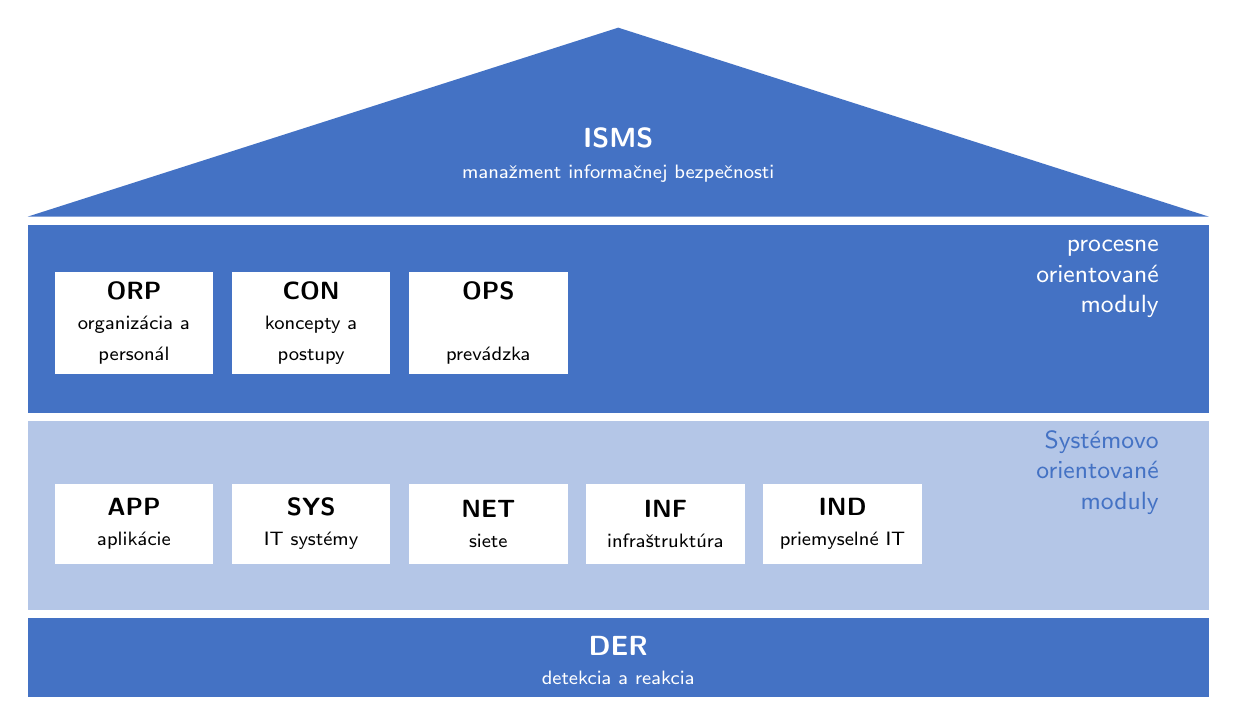
\begin{tikzpicture}[
    every node/.style={font=\sffamily},
    box/.style={
        rectangle,
        draw=white,
        fill=white,
        minimum width=2.0cm,
        minimum height=1.0cm,
        align=center,
        font=\sffamily\small
    }
]

\definecolor{midblue}{RGB}{68, 114, 196}
\definecolor{lightblue}{RGB}{180, 198, 231}

\fill[midblue] (0, 0) rectangle (15, 1.0);
\node[text=white, font=\sffamily\bfseries] at (7.5, 0.65) {DER};
\node[text=white, font=\sffamily\scriptsize] at (7.5, 0.25) {detekcia a reakcia};

\fill[lightblue] (0, 1.1) rectangle (15, 3.5);
\node[text=midblue, font=\sffamily\small, anchor=north east] at (14.7, 3.55)
    {\begin{tabular}{r}Systémovo\\orientované\\moduly\end{tabular}};
\node[box] at (1.35,  2.2) {\textbf{APP}\\\scriptsize aplikácie};
\node[box] at (3.6,   2.2) {\textbf{SYS}\\\scriptsize IT systémy};
\node[box] at (5.85,  2.2) {\textbf{NET}\\\scriptsize siete};
\node[box] at (8.1,   2.2) {\textbf{INF}\\\scriptsize infraštruktúra};
\node[box] at (10.35, 2.2) {\textbf{IND}\\\scriptsize priemyselné IT};

\fill[midblue] (0, 3.6) rectangle (15, 6.0);
\node[text=white, font=\sffamily\small, anchor=north east] at (14.7, 6.05)
    {\begin{tabular}{r}procesne\\orientované\\moduly\end{tabular}};
\node[box] at (1.35,  4.75) {\textbf{ORP}\\\scriptsize organizácia a \\\scriptsize personál};
\node[box] at (3.6, 4.75) {\textbf{CON}\\\scriptsize koncepty a\\\scriptsize postupy};
\node[box] at (5.85,  4.75) {\textbf{OPS}\\\\\scriptsize prevádzka};

\fill[midblue] (0, 6.1) -- (7.5, 8.5) -- (15, 6.1) -- cycle;
\node[text=white, font=\sffamily\bfseries] at (7.5, 7.1) {ISMS};
\node[text=white, font=\sffamily\scriptsize] at (7.5, 6.65) {manažment informačnej bezpečnosti};


\end{tikzpicture}
\caption{Vrstvový model, prevzatý z \cite{GSK} a upravený, tmavomodré pozadie sú procesné moduly a bledomodré pozadie sú systémove moduly.}
\label{fig:gsk-layer-model}
\end{figure}

V rámci tejto práce budeme uvádzať príklady najmä zo systémovo-orientovaných modulov, nakoľko k ním máme najbližšie. Vrstvu DER spomenieme iba
okrajovo, keďže súvisí s kontrolou bezpečnostných opatrení, detekciou a reakciou na bezpečnostné incidenty, čo je mimo náš rozsah.

Pred tým, ako prejdeme k analýze rizík, venujeme ešte jednu sekciu politiku KIB, kde čitateľovi v krátkosti vysvetlíme jej význam, vzhľadom
na to, že jej obsah ovplyvňuje vstup a výsledok analýzy rizík a naopak, výsledky analýzy rizík môžu iniciovať zmenu politiky.

\section{Politika informačnej bezpečnosti}
Politika informačnej bezpečnosti je jedným z kľúčových dokumentov organizácie, ktorého účelom je vo všeobecnosti popísať, akým spôsobom má byť
zriadená informačná bezpečnosť v organizácii. Je to rámcový dokument, ktorý vymedzuje účel, zdroje a štruktúru informačnej bezpečnosti, pričom
stanovuje ciele a opisuje požadovanú úroveň informačnej bezpečnosti, ktorú sa organizácia pokúša dosiahnuť. Spôsob, ktorým plánuje organizácia
dosiahnuť deklarovaný obsah, je rozvinutý v bezpečnostnej stratégii.

\subsection*{Príprava politiky}
 
Vedenie organizácie musí prebrať zodpovednosť za informačnú bezpečnosť, ďalším krokom je vytvoriť tím na vyvinutie politiky. Do tohto procesu
potrebujeme zakomponovať zamestnancov zodpovedných za organizačné celky aj ľudí kvalifikovaných v informačnej bezpečnosti. Odborné znalosti
môžeme čerpať napr. od IT špecialistov, ľudských zdrojov, audítorov alebo právneho oddelenia. Návrh a finálne znenie politiky predkladáme
vedeniu organizácie, ktoré ju schvaľuje.

\subsection*{Rozsah a obsah politiky}

Politika explicitne vymedzuje rámec pôsobností, teda či sa aplikuje na celú organizácie alebo vybrané organizačne celky. Obsah politiky
by mal byť čo najstručnejší a jasne formulovaný, nemali by sme sa pokúšať vyrobiť príliš rozsiahly dokument, vzhľadom na to, že obsah
a požiadavky by mali byť jasné a zrozumiteľné každému zamestnancovi, bez ohľadu na pracovné obsadenie. Politika by mala ponúkať
odpovede na tieto otázky:
\begin{itemize}[nosep]
        \item Akú hodnotu má informačná bezpečnosť?
        \item Aké dôležité sú informácie, dáta, biznisové procesy, informačné systémy pre plnenie poslania organizácie?
        \item Aké sú bezpečnostné ciele a kľúčové prvky bezpečnostnej stratégie pre organizáciu?
        \item Aký je vzťah cieľov informačnej bezpečnosti vzhľadom na poslanie organizácie?
        \item Aká organizačná štruktúra bola zriadená na podporu bezpečnostného procesu?
        \item Aké sú najväčšie hrozby, ktorým naša organizácia čelí?
        \item Aké sú esenciálne úlohy, kompetencie a roly bezpečnostného procesu?
        \item Aké kroky naša organizácia podnikne na zvyšovanie povedomia o informačnej bezpečnosti?
\end{itemize}

\subsection*{Oboznámenie a aktualizácia politiky}

O existencii politiky potrebujeme oboznámiť všetkých (aj nových) zamestnancov, politiku musíme zverejniť na ľahko prístupnom mieste.
Keďže v politike sú obsiahnuté nové úlohy a záväzné povinnosti, zamestnanci musia rozumieť jej obsahu, aby im bolo jasné, čo od nich
požadujeme a očakávame. Rovnako aj prípadné sankcie, ktoré im budú uložene v prípade porušovania/nedodržiavania politiky. V pravidelných
intervaloch revidujeme obsah politiky (každý rok alebo každé dva roky alebo v prípade výnimočnej udalosti), aby sme sa systematicky
prispôsobovali interným zmenám (napr. procesov, úloh, procedúr alebo komponentov) a externým zmenám (napr. legislatívy, technológií
alebo globálnych hrozieb).
